\documentclass[a4paper]{jarticle}
\usepackage{comment}
\usepackage[top=20truemm,bottom=20truemm,left=20truemm,right=20truemm]{geometry}
\usepackage[dvipdfmx]{graphicx}
\usepackage[utf8]{inputenc}
\title{ソフトウェア工学レポート084}
\author{学生番号 氏名}
\date{\today}
\begin{document}
\maketitle
\begin{enumerate}
 \renewcommand{\labelenumi}{(\arabic{enumi})}
 \item 「情報コース ミニライブラリ(仮称) 仕様 v3」のデータ項目とWBSを作成してください。
 \begin{itemize}
  \item データ項目\\
\begin{comment}
v2データ項目
利用者はアカウントを持つ
アカウントデータの項目はメールアドレス、教員/学生の区別、パスワードである
学生アカウントは指導教員アカウントを持つ
図書室の書架のぞれぞれに書架番号がつけられている
各書籍には一冊ずつ番号(書籍番号)がつけられる
書籍データの項目は書籍番号、ISBN、著者、タイトル、出版社、発行年、所有する教員のアカウント、書架番号である
大学図書館の書籍に関しては、さらに、大学図書館の管理番号が記録されている
貸出データの項目は、貸出中の書籍ごとに、書籍番号、貸出開始日時、貸出先アカウント
予約データの項目は、予約ごとに、書籍番号、予約日時、予約者のアカウント(同じ書籍に対する予約が複数存在することがある)
\end{comment}
利用者はアカウントを持つ\\
アカウントデータの項目はメールアドレス、教員/学生の区別、パスワード、アカウントが有効か無効かを示すフラグである\\
学生アカウントは指導教員アカウントを持つ\\
図書室の書架のぞれぞれに書架番号がつけられている\\
各書籍には一冊ずつ番号(書籍番号)がつけられる\\
書籍データの項目は書籍番号、ISBN、著者、タイトル、出版社、発行年、所有する教員のアカウント、書架番号である\\
大学図書館の書籍に関しては、さらに、大学図書館の管理番号が記録されている\\
貸出データの項目は、貸出中の書籍ごとに、書籍番号、貸出開始日時、貸出先アカウント\\
予約データの項目は、予約ごとに、書籍番号、予約日時、予約者のアカウント(同じ書籍に対する予約が複数存在することがある)\\
  \item WBS\\
\begin{comment}
v2WBS
WBSのうち、ソフトウェア・システムの分解の部分
アカウント管理
アカウントテーブル
アカウント新規作成機能(管理者は、アカウントを新規作成することができる)
アカウント削除機能(管理者は、アカウントを削除することができる)
アカウント修正機能(利用者は、自分自身のアカウントのパスワードを修正することができる)
アカウント管理UI
蔵書管理
書籍テーブル
書籍登録機能(教員は、新規に書籍を登録できる。このとき書架番号も同時に登録する)
書籍抹消機能(教員は、自分自身が所有する書籍の登録を抹消できる)
蔵書管理UI
貸出・返却・予約管理
貸出テーブル
予約テーブル
予約貸出機能(教員は、ある書籍について、予約日時が一番古い予約者の指導教員が自分自身であるとき、または、予約者が自分自身であるとき、その書籍をその予約者が借りている状態にできる。ただし、すでに貸出中の書籍についてはこの処理を行うことはできない)
即時貸出機能(教員は、ある書籍について、貸出中でも予約中でもなければ、書籍を自分自身が借りている状態にすることができる)
返却機能(教員は、自分が貸出処理を行った貸出中の書籍を借りられていない状態にすることができる)
一覧機能(利用者は、すべての書籍について、書籍の著者やタイトルなど、書架番号、および、予約中/貸出中の一覧を見ることができる)
予約機能(利用者は、書籍を予約することができる。学生が予約した場合には、指導教員に催促するメールが送られる)
予約状況更新機能(ある書籍が貸出中ではないが、予約中である状態が3日以上続いたときには、その書籍の一番古い予約が削除される。貸出中ではない期間が続く間、3日ごとに一番古い予約がされる。)
貸出・予約UI
返却UI
セッション管理
ログイン機能(利用者はパスワード認証によりシステムにログインできる。上述のすべての機能はログインしてから操作するものとする)
ログアウト機能(ログイン中の利用者はシステムからログアウトできる)
\end{comment}
WBSのうち、ソフトウェア・システムの分解の部分
  \begin{itemize}
   \item アカウント管理
    \begin{itemize}
     \item アカウントテーブル
     \item アカウント新規作成機能(管理者は、アカウントを新規作成することができる)
     \item アカウント無効化機能(管理者は、アカウントを無効化することができる)
     \item アカウント修正機能(利用者は、自分自身のアカウントのパスワードを修正することができる)
     \item アカウント管理UI
    \end{itemize}
   \item 蔵書管理
    \begin{itemize}
     \item 書籍テーブル
     \item 書籍登録機能(教員は、新規に書籍を登録できる。このとき書架番号も同時に登録する)
     \item 書籍抹消機能(教員は、自分自身が所有する書籍の登録を抹消できる)
     \item 蔵書管理UI
    \end{itemize}
   \item 貸出・返却・予約管理
    \begin{itemize}
     \item 貸出テーブル
     \item 予約テーブル
     \item 予約貸出機能(教員は、ある書籍について、予約日時が一番古い予約者の指導教員が自分自身であるとき、または、予約者が自分自身であるとき、その書籍をその予約者が借りている状態にできる。ただし、すでに貸出中の書籍についてはこの処理を行うことはできない)
     \item 即時貸出機能(教員は、ある書籍について、貸出中でも予約中でもなければ、書籍を自分自身が借りている状態にすることができる)
     \item 返却機能(教員は、自分が貸出処理を行った貸出中の書籍を借りられていない状態にすることができる)
     \item 一覧機能(利用者は、すべての書籍について、書籍の著者やタイトルなど、書架番号、および、予約中/貸出中の一覧を見ることができる)
     \item 予約機能(利用者は、書籍を予約することができる。学生が予約した場合には、指導教員に催促するメールが送られる)
     \item 予約状況更新機能(ある書籍が貸出中ではないが、予約中である状態が3日以上続いたときには、その書籍の一番古い予約が削除される。貸出中ではない期間が続く間、3日ごとに一番古い予約がされる。)
     \item 予約キャンセル機能(予約者は、自分がした予約をキャンセルすることができる。)
     \item 貸出・予約UI
     \item 返却UI
    \end{itemize}
   \item セッション管理
    \begin{itemize}
     \item ログイン機能(利用者はパスワード認証によりシステムにログインできる。上述のすべての機能はログインしてから操作するものとする)
     \item ログアウト機能(ログイン中の利用者はシステムからログアウトできる)
    \end{itemize}
  \end{itemize}
 \end{itemize}
 \item v3のデータフローダイアグラムのうち、次の機能に関わるものを新規作成してください。 次の機能のうち、v2のデータフローダイアグラムにも存在するものに関しては、v3の機能に合わせて修正してください。
 \begin{itemize}
  \item アカウント無効化機能
  \item 予約貸出機能
  \item 即時貸出機能
  \item 返却機能
 \end{itemize}
 \begin{center}
 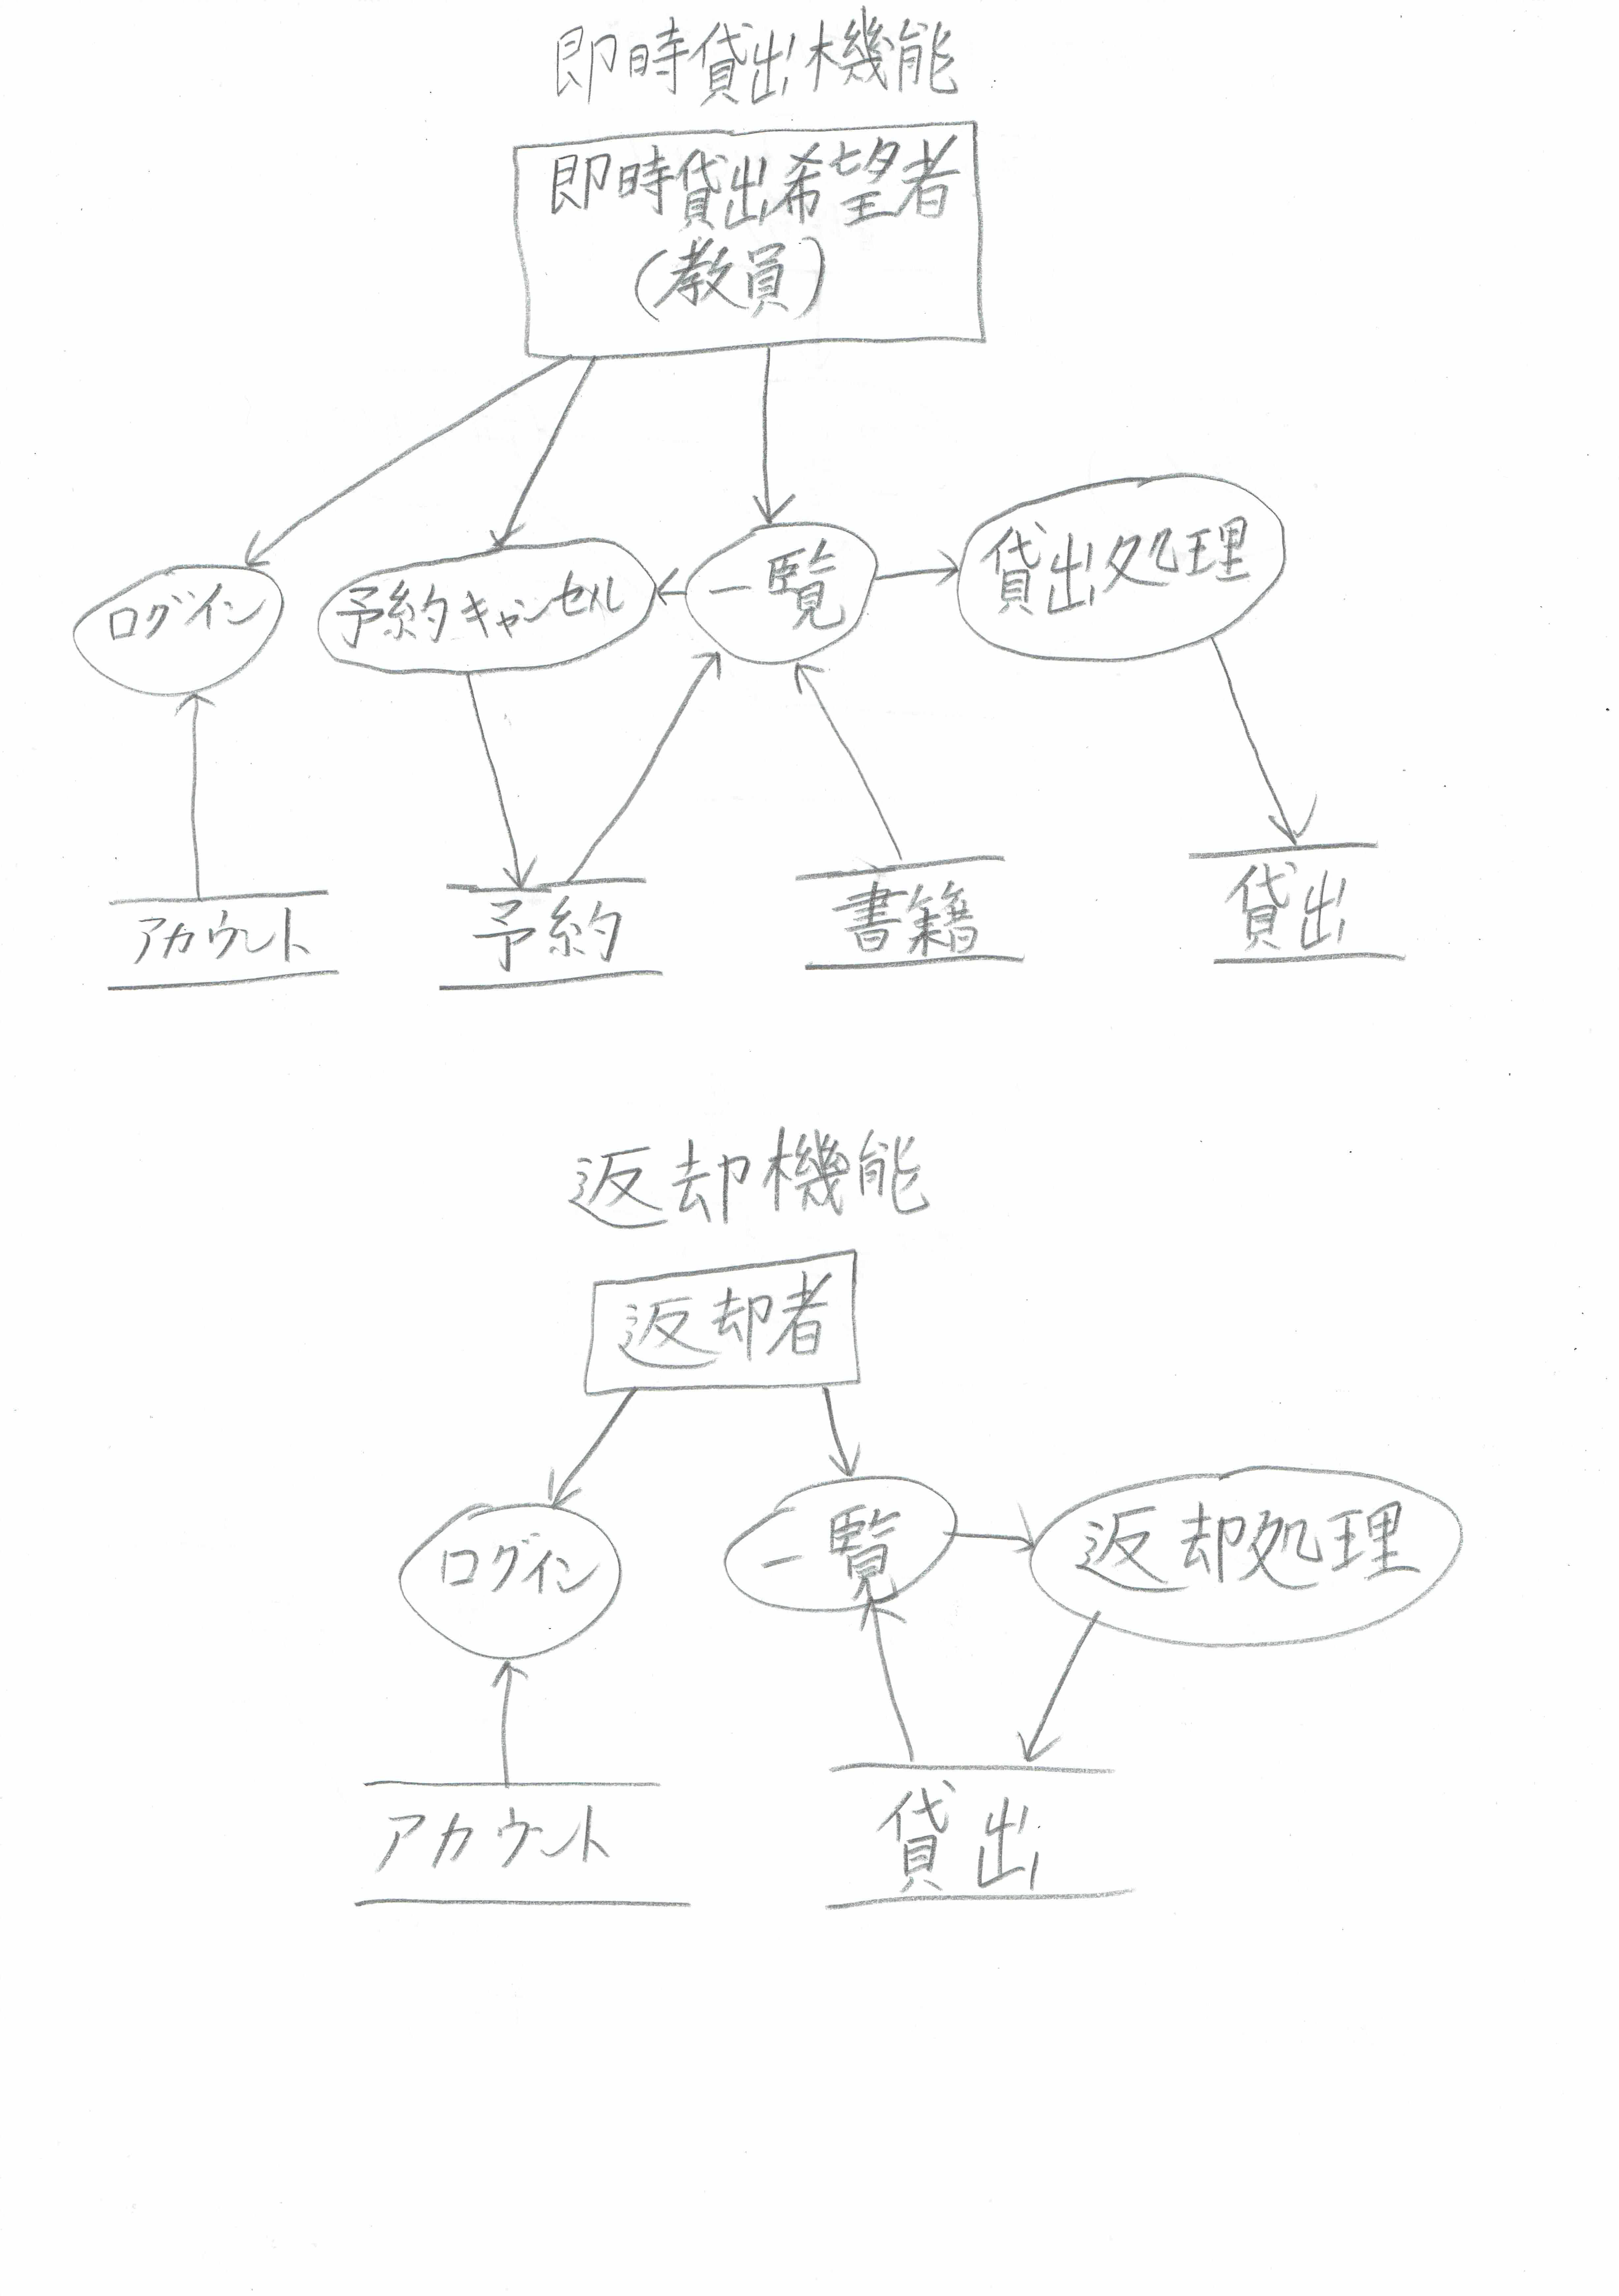
\includegraphics[width=15cm]{DFD1.JPG}
 \end{center}
 \begin{center}
 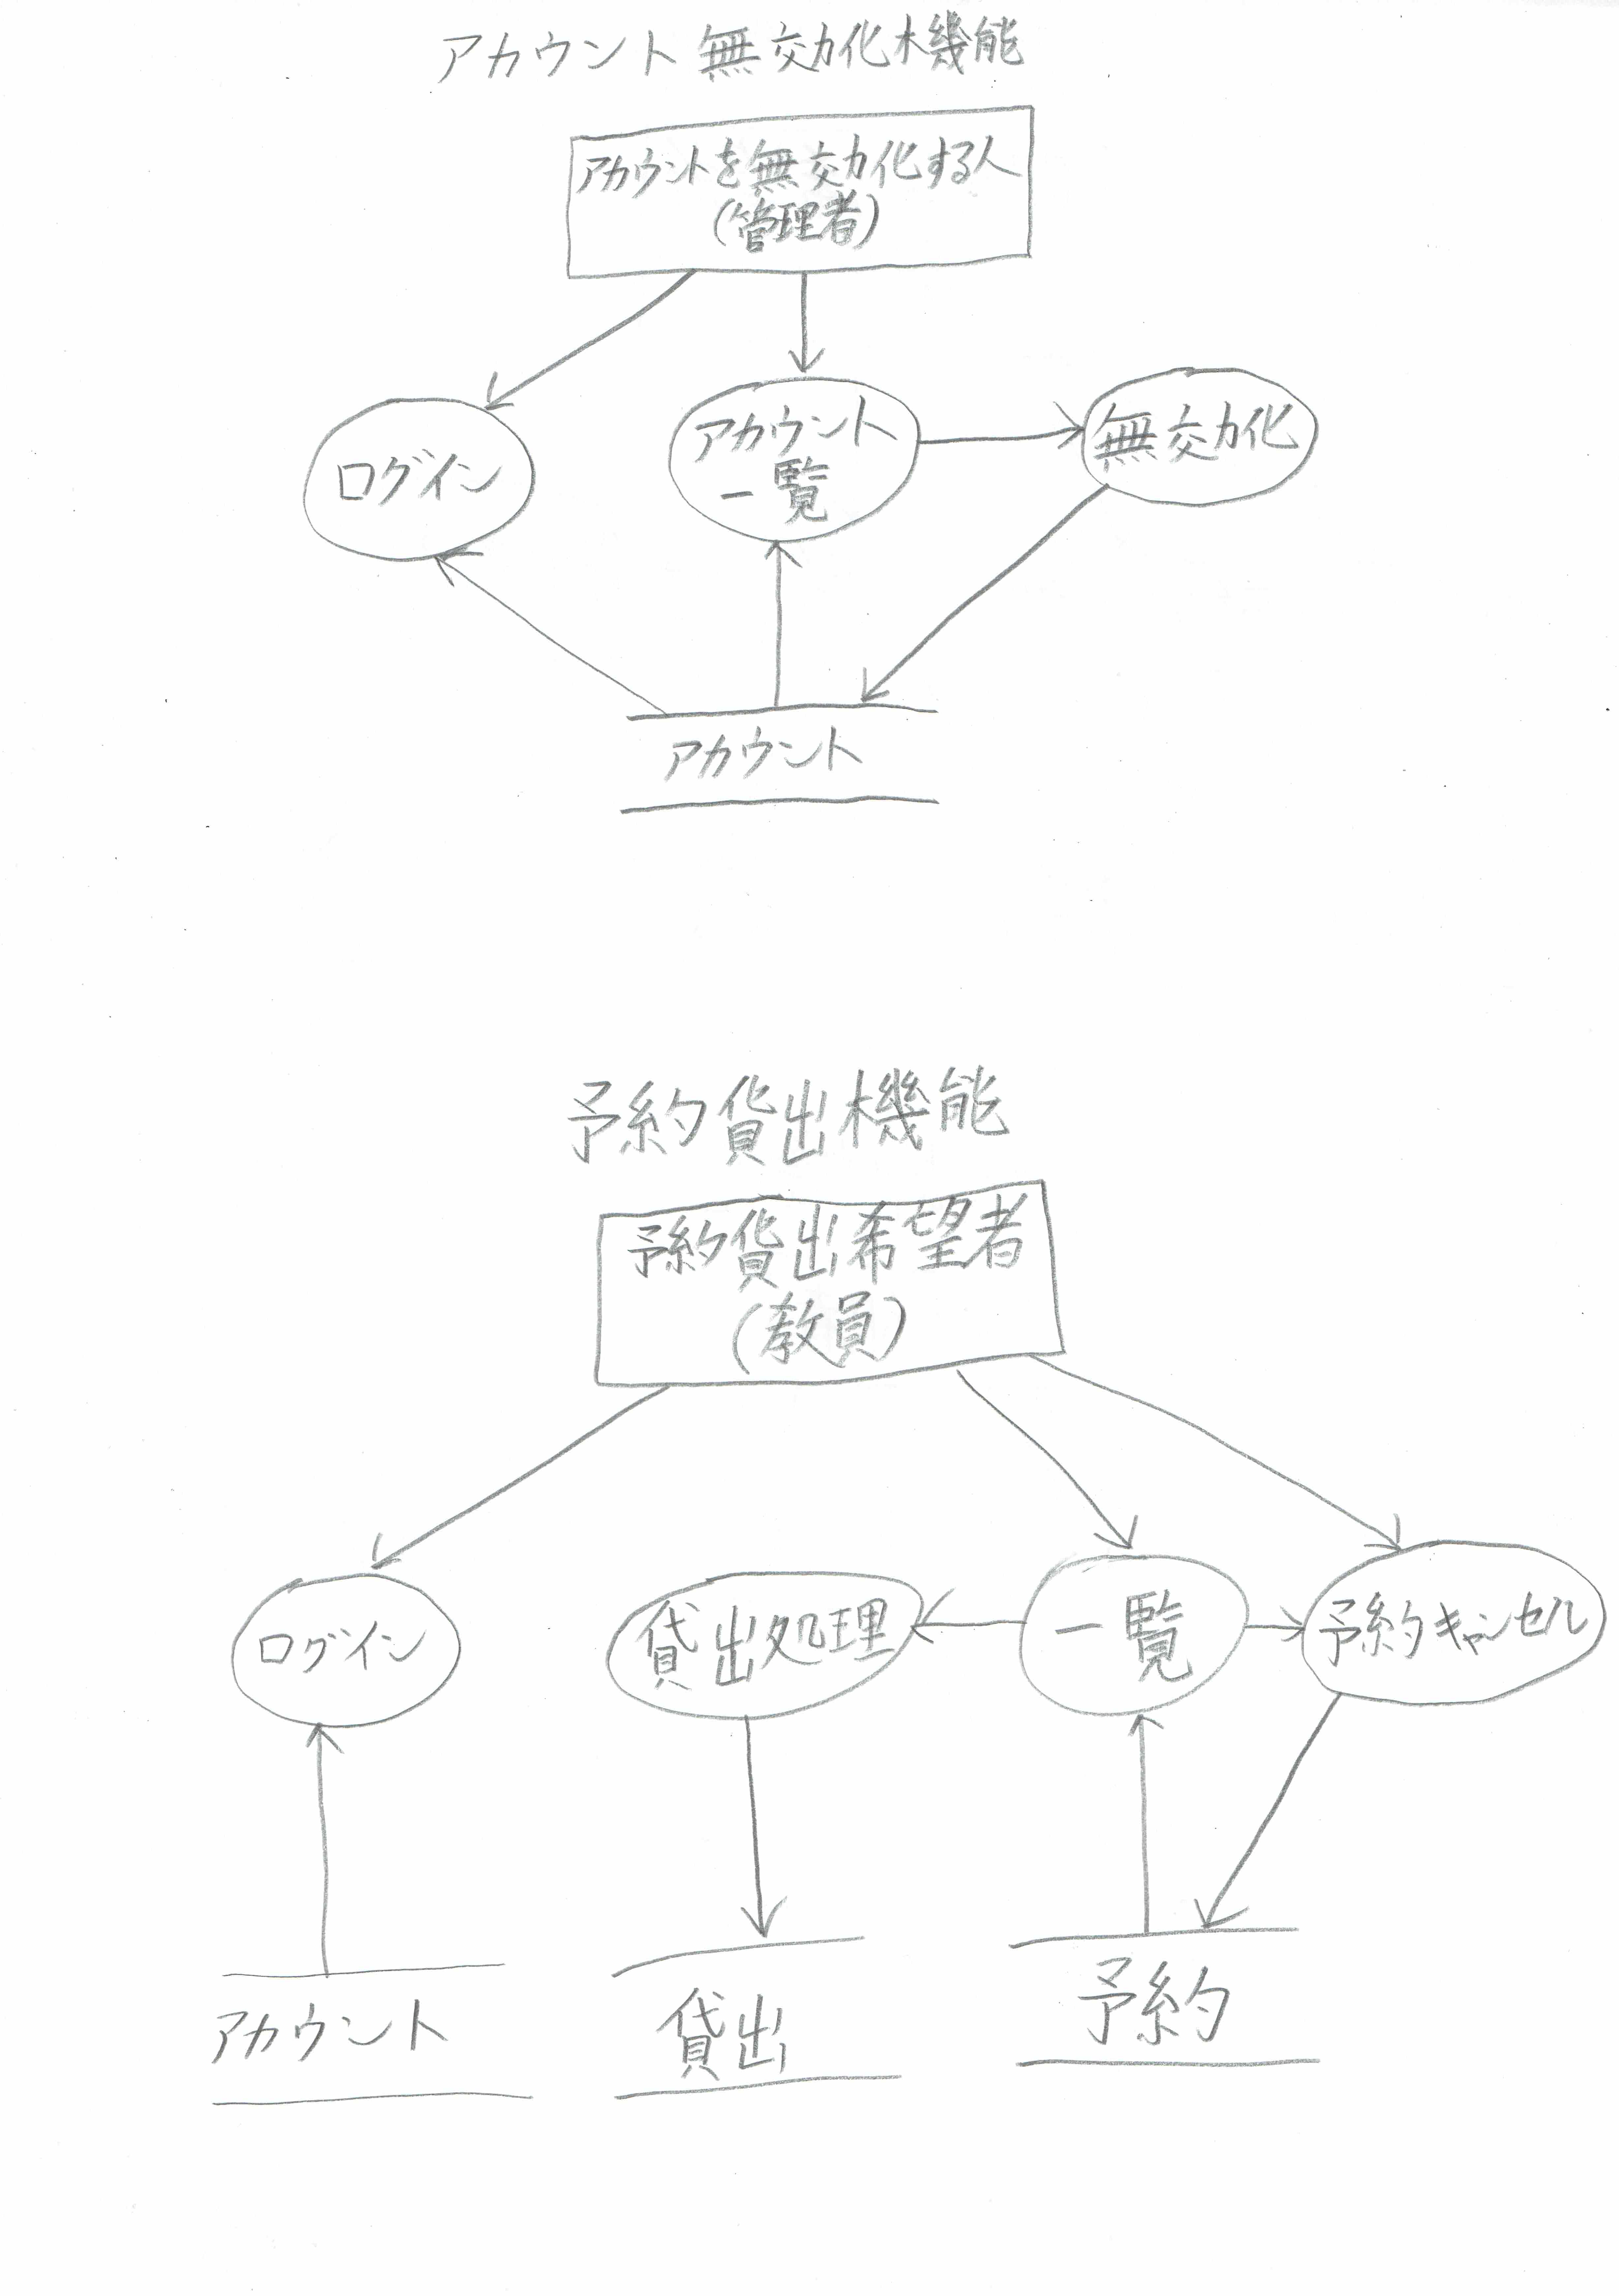
\includegraphics[width=15cm]{DFD2.JPG}
 \end{center}
\end{enumerate}
\end{document}
